\section{The Complicity Spiral: How to Make Everyone Dirty So No One Can Cleanly Leave}

\vfill


\begin{figure}[H]
  \centering
  
  % === First row ===
  \begin{subfigure}[t]{0.45\textwidth}
  \centering
  \begin{tikzpicture}
    \comicpanel{0}{0}
      {Centauri Exec}
      {Aurora Founder}
      {Tonight’s not about contracts. It’s about belonging.}
      {(-0.6,-0.6)}
  \end{tikzpicture}
  \caption*{The invitation: ambiguous, alluring, loaded.}
  \end{subfigure}
  \hfill
  \begin{subfigure}[t]{0.45\textwidth}
  \centering
  \begin{tikzpicture}
    \comicpanel{0}{0}
      {Centauri Exec}
      {Aurora Founder}
      {Belonging to what?}
      {(0.6,-0.6)}
  \end{tikzpicture}
  \caption*{The hesitation: unease creeping beneath the promise.}
  \end{subfigure}
  
  \vspace{1em}
  
  % === Second row ===
  \begin{subfigure}[t]{0.45\textwidth}
  \centering
  \begin{tikzpicture}
    \comicpanel{0}{0}
      {Centauri Exec}
      {Aurora Founder}
      {The "group". Everyone in that room’s done each other favors. That’s why it works.}
      {(-0.6,-0.6)}
  \end{tikzpicture}
  \caption*{The reassurance: a quiet implication of reciprocity.}
  \end{subfigure}
  \hfill
  \begin{subfigure}[t]{0.45\textwidth}
  \centering
  \begin{tikzpicture}
    \comicpanel{0}{0}
      {Centauri Exec}
      {Aurora Founder}
      {And what if I don’t want to owe anyone favors?}
      {(0.6,-0.6)}
  \end{tikzpicture}
  \caption*{The warning: a question asked too late.}
  \end{subfigure}
  
  \caption*{In some rooms, the price of entry isn’t on the invitation. It’s in the tab you don’t know you’re running.}
\end{figure}



\subsection{The Prologe}

The glow of David’s laptop cast long shadows across the quartz countertop. He was still in his dress shirt, sleeves rolled, 
tie forgotten somewhere in the house. Slide 14 was open again. ``Risk Stratification Under Uncertainty.'' He adjusted a 
chart’s axis, then stared at it like it had betrayed him.

Behind him, the hallway light flicked on.

``You said no more of this,'' Emma said from the doorway.

David didn’t look up. ``It’s just one last push.''

``You said that last week. And the week before.''

``This one’s different. I’m speaking tomorrow. The conference panel—''

``—doesn’t tuck the kids in,'' she cut in.

She walked to the fridge, opened it, stared blankly. A bottle of wine shifted when she grabbed the door. She didn’t take it.

``You promised this would be better,'' she said. ``That starting your own thing meant more time. Not... whatever this is.''

He sighed. ``You know this is for us, right? The whole point is—''

``You’re pitching to your wife at two in the morning. Do you hear yourself?''

He finally turned. ``I’m trying to build something that lasts.''

Emma leaned on the counter, arms folded. ``What if we already had something that lasts, and you're too busy optimizing 
it into oblivion?''

He didn’t answer. She glanced at the screen.

``Let me guess. Twenty-five slides, zero about what it’s costing you.''

``It’s costing us now so it doesn’t later.''

She looked at him the way people look at someone they love when they’re quietly writing a different ending.

``Just... don’t sell your soul.''

David smiled tiredly. ``I’m not selling anything.''

``That’s what makes it scarier,'' she said, and left the room.

The silence settled in behind her like fog. He sat still for a moment, blinking.

Then, quietly, he deleted the phrase ``adaptive resilience'' and typed \textbf{``Compliant AI Infrastructure for Enterprise Risk.''}

He stared at it. Then clicked save.

\subsection{The Conference}

Michael Hart was in the audience.

Technically, he wasn’t supposed to be at the conference. But a client meeting had fallen through, and he figured he’d kill 
the day at the conference. 

Hart listened.  He leaned forward. And by the second case study, he knew.

Afterward, he walked straight up to David. Hart had no pitch deck. He had no small talk.

“I’ve got distribution,” Hart said. “You’ve got product.”

He handed David a business card and said “Let’s talk.”

Hart was the founder of Centauri Consulting which billed itself as “the velvet glove of high-stakes transformation.” 
He didn’t just sell strategic roadmaps: he sold access. His firm specialized in landing contracts others couldn’t 
touch (i.e. complex, high-margin deals requiring deep ties to institutional investors, regulators, and 
public-private partnerships).

But Centauri wasn’t just looking for clients. It was looking for \textbf{technical talent it couldn’t poach outright}.

\medskip

\begin{HistoricalSidebar}{The Dark Side of Acquihires --- When Talent Becomes Leverage}

  In the early 2000s, as Silicon Valley’s war for engineering talent reached fever pitch, a new acquisition model 
  quietly took over the startup ecosystem: the \textbf{acquihire}.

  \medskip
  
  Unlike a traditional acquisition, where the buyer wants the product, patents, or market share, an acquihire’s primary 
  target is \textbf{the team}. The startup itself might be shut down, its technology shelved, its users abandoned. The 
  engineers were the real asset.

  \medskip
  
  At first, acquihires were framed as \textit{soft landings} for struggling startups—a face-saving way to pay back 
  investors, a lifeboat for founders, a pathway into Big Tech.

  \medskip
  
  But beneath the glossy press releases, a harsher reality unfolded.

  \medskip
  
  Founders often found themselves negotiating from a position of desperation, their options underwater, their runway gone. 
  Investors pressured them to “return something” rather than risk a total wipeout. Engineers were given golden handcuffs: 
  lucrative retention bonuses tied to multi-year employment agreements, conditional on project milestones that conveniently 
  reset their vesting clocks.

  \medskip
  
  In some cases, acquihires functioned as \textbf{talent raids disguised as mergers}. A competitor could eliminate a rival’s 
  core team while burying its roadmap. A corporation could sidestep a hiring freeze by acquiring headcount off the books.

  \medskip
  
  And for founders, the acquihire wasn’t always an exit—it was a quiet exile.
  
  \medskip
  
  The deeper lesson?

  \medskip
  
  An acquihire doesn’t just buy talent. It \textbf{absorbs leverage}. It converts independent actors into vested stakeholders, 
  ties reputations to institutional outcomes, and rewrites incentives through retention clauses and non-compete agreements.
  Because The real deal isn’t written in the press release.  The real deal is written in the clauses that keep you from leaving.
  
\end{HistoricalSidebar}

\medskip

\subsection{The Partnership Structure}

Hart proposed a partnership:  
Aurora would provide the technical muscle — developers, protocol engineers, and product interfaces.  
Centauri, with its deep institutional Rolodex, would unlock high-level enterprise and government engagements.

\medskip

On paper, it was a perfect match:  
\begin{itemize}
  \item Aurora brought the code.  
  \item Centauri brought the clients.  
  \item Both would share the upside.
\end{itemize}

\medskip

Legally, they structured it as a joint venture under a Delaware LLC shell, with:
\begin{itemize}
  \item \textbf{50/50 profit split} after cost recovery.
  \item \textbf{Aurora} holding IP rights to the core protocol and payment infrastructure.
  \item \textbf{Centauri} owning the exclusive licensing rights for specific verticals (e.g., defense, health data, cross-border finance).
  \item \textbf{Liability firewalling} between code execution and client delivery — Aurora would not be legally responsible for how Centauri sold or implemented the tech stack.
\end{itemize}

\medskip

The arrangement gave Aurora plausible deniability in client matters  
and gave Centauri a ready-made infrastructure without needing to staff an engineering team.

\begin{quote}
\textit{The ideal compromise — or the perfect diffusion of responsibility.}
\end{quote}


\medskip

\begin{figure}[H]
  \centering
  \begin{tikzcd}[row sep=huge, column sep=huge, ampersand replacement=\&]
    \textbf{Aurora Labs} \arrow[rd, "Technology + IP"'] \& \& \textbf{Centauri Partners} \arrow[ld, "Licensing + Access"] \\
    \& \boxed{\text{Aurora–Centauri JV (Delaware LLC)}} \arrow[d, "Deployment + Monetization"] \& \\
    \& \textbf{Clients (Enterprise + Gov)} \& 
  \end{tikzcd}
  \caption{Commutative Diagram of the Aurora–Centauri Joint Venture Structure}
\end{figure}

\medskip

David and Hart met for drinks that night in the hotel bar with Alex joining midway through. Hart sketched their partnership 
on a napkin between whiskey refills. Aurora would bring the algorithms. Centauri would bring the clients. They’d split 
the contracts down the middle.

But Hart didn’t jump straight to business. Not this time. 

Hart was a storyteller, a collector of details. Between strategy talk and scribbled numbers, he asked about the company’s origin. 
Hart asked about how Alex and David had met. Hart asked about what it was like building a business together. 
Hart asked about how they’d kept the friendship intact through the stress.

Hart smiled when David mentioned his wife. 

“She must be a saint to put up with a startup guy,” Hart joked while raising his glass. “You two must be adorable together,”
he continued. 

Hart asked how they met, how long they’d been married, and whether they 
planned to start a family.

To David, it didn’t feel invasive. To David, it felt friendly. To David, it felt easy.  

By the second round, David felt like he’d known Micheal for years.

Hart didn’t just want to know the business.  
Hart wanted to know the people behind it.  
And by the time David and Micheal clinked glasses over the napkin contract,  
their meeting didn’t feel like a negotiation.  
It felt like a friendship.

Looking back, David would realize that Hart had gathered more than stories that night.  
He’d gathered leverage.

\medskip

\begin{PsychologicalSidebar}{The Thin Line Between Help and Grooming}

  Psychologists use the term \textbf{grooming} to describe the process by which a more powerful actor builds trust, 
  dependency, and emotional leverage over a target—incrementally lowering their resistance to boundary violations.

  \medskip
  
  While often discussed in interpersonal or criminal contexts, the same psychological mechanisms can surface in 
  professional and institutional settings.

  \medskip
  
  At its core, grooming is a strategy of \textbf{gradual normalization}:  

  \begin{itemize}
    \item Each “favor” feels like mentorship.  
    \item Each private invitation feels like inclusion.  
    \item Each off-the-record conversation feels like trust.
  \end{itemize}

  \medskip
  
  But beneath the veneer of help lies a quiet asymmetry. The powerful actor controls access, opportunity, and escalation. 
  The recipient is positioned to feel indebted, grateful, increasingly reluctant to say no.

  \medskip
  
  In Centauri’s partnership with Aurora, the grooming wasn’t sexual or criminal—it was structural. Every dinner, every 
  introduction, every off-paper meeting created a subtle but compounding sense of \emph{obligation}.
  
  \begin{quote}
  Grooming is effective not because it overtly coerces,  but because it makes resistance feel like betrayal.
  \end{quote}
  
  The psychological danger is that the line between help and manipulation isn’t marked by intent—it’s marked by 
  \textbf{power asymmetry and conditionality}.  When help comes bundled with escalating asks, unstated expectations, 
  and deferred reciprocation, it stops being help.  It becomes preparation.
  
\end{PsychologicalSidebar}

\medskip

On paper, it was a perfect match.  In the moment, it felt like destiny.  And in hindsight, it was the first move in a 
game Aurora didn’t realize they were playing.

\subsection{The Pattern They Never Taught in Startup School}

At first, everything felt above board.

\begin{itemize}
  \item Centauri brought Aurora into key meetings.  
  \item Centauri introduced them to regulators at roundtable panels.  
  \item Centauri helped them polish their pitch decks for institutional audiences.  
  \item Centauri invited them to private dinners after conferences.
\end{itemize}

Micheal Hart positioned everything as mentorship, sponsorship, or partnership.

Then came the quiet invitations.

Each gesture felt like a reward. Each night felt earned. Each invitation felt like trust.
Each invitation pulled them closer together. Each gathering made the room feel warmer, 
smaller, and more intimate.  

\textbf{Every event pulled them a step deeper into... ``the lifestyle.''}

\medskip

\begin{HistoricalSidebar}{\textit{“The Lifestyle”} --— A System, Not Just a Scene}

  “The lifestyle” isn’t a formal organization, and it’s not a job description. It’s a term whispered in 
  back rooms, joked about in group chats, and nodded to in memoirs. It's a euphemism with just enough 
  ambiguity to survive deniability.

  \medskip
  
  But its structure is older than the name.
  
  \medskip
  
  The phrase \textbf{originated in postwar finance and law circles}, where rising partners in New York 
  or London learned there were rules that weren’t written in any handbook:

  \medskip
  
  \begin{itemize}
    \item Where to eat, and who picks up the check.
    \item What to say at the fundraiser, and how much to donate.
    \item Who to toast, who to avoid, and who to “owe.”
  \end{itemize}

  \medskip
  
  In the 1960s and ’70s, as global capital markets expanded and high-stakes consulting emerged as its own discipline, 
  “the lifestyle” became a shorthand for the invisible initiation into elite trust networks. It became a set of habits, 
  indulgences, and obligations that \textbf{blurred the line between client, colleague, and co-conspirator}.
  
  \medskip
  
  It’s not just about luxury.

  \medskip
  
  It’s about shared rituals: the invite-only dinner after the conference, the private box at the regatta, the sudden 
  overseas “work trip” that doesn’t make it onto the ledger.
  
  \medskip
  
  It’s called a lifestyle because once you’re in, it’s no longer “extra.” It becomes the air you breathe. And that’s 
  the point.
  
  \begin{quote}
    \textit{You don’t just do business with someone in the lifestyle.} \
    \textit{You live inside a mutual web of favors, memories, and quiet debts.}
  \end{quote}

  \medskip
  
  What makes it durable isn’t that it’s hidden.  It’s that it’s \textbf{normalized}.

  \medskip
  
  No one says, “Welcome to the lifestyle.” They just keep inviting you back.
  
  \medskip
  
  Culturally, “the lifestyle” functions like a soft cartel. However, it is not one built on explicit price-fixing, 
  but on access-fixing. It is a velvet caste system where reputations, introductions, and loyalty are currency.
  
  \medskip
  
  Legally, it skirts the edges:
  It's not bribery. It's just hospitality.
  It's not coercion. It's just culture.
  It's not blackmail. It's just memory.
  
  \medskip
  
  And once you’re in, leaving isn’t just hard. It’s suspicious.  Because when you exit the lifestyle...  
  you make a statement by doing so.
  
\end{HistoricalSidebar}

\medskip


What Aurora’s founders didn’t see was the pattern.

It started with a private tasting at a members-only club in Manhattan, where the sommelier greeted Hart by name and poured from bottles “not on the menu.” David Hart had barely touched his first glass when a white-gloved waiter brought out a vintage Côte-Rôtie “courtesy of Mr. Colburn.” Hart hadn’t heard the name before, but everyone else at the table had.

Then came a last-minute seat at a soft-launch dinner in D.C., surrounded by policy advisors, consultants, and a few ex-State Department operatives who traded rumors like currency between courses. Somewhere between the second and third pour, one of the members leaned over and murmured with a wink:  
\begin{quote}
  Didn’t realize we both shared the same unicorn.
\end{quote}  
David laughed reflexively, unsure whether it was a startup reference or a euphemism. He didn’t ask.

\medskip

A few weeks later came a casual poker night — “just the inner circle, nothing serious” — hosted in a stone-and-glass penthouse overlooking the river. The stakes weren’t really money. They were favors, confessions, quiet nods across the table. David folded early and watched.

Someone mentioned, offhand, how two partners had swapped wives at last quarter’s offsite in Jackson Hole.  
What shocked David wasn’t the story — it was that no one reacted. No laughter. No discomfort. Just a shrug, and another pour.

\medskip

The moment it clicked was in the velvet booth at Chambre Noire, an invitation-only lounge in Mayfair.

They were “celebrating a win,” which in this circle meant a lobbyist deal had gone through. Hart leaned in, 
a little too relaxed, and casually dropped the line:

\begin{quote}
  Serena and I stayed over at Colburn’s place last night. Brought Mia, of course.
\end{quote}

He said it like one might mention a bottle of wine. Mia... that was the unicorn.  

Mia wasn’t just beautiful; she was disarming, curious, and fluent in four languages. Her role wasn’t transactional. 
She made people feel seen... including the wives. She had an unnerving talent for anchoring awkward silences and 
smoothing over taboos with a knowing smile. She wasn’t owned, but she was shared. She was  a symbol of access, trust, 
and mutual blackmail.

She moved quietly through the inner rings of Centauri’s network, a constant presence but never in focus. Always invited, 
never named in the minutes.  

\medskip

By the time David connected the dots, he was already too deep to leave without causing a scene.  
And in this world, scenes were remembered.


\medskip

\begin{HistoricalSidebar}{The Unicorn --- The Other Kind of Startup Fantasy}

  In modern swinger and polyamorous circles, a \textit{unicorn} refers to a single, bisexual woman willing to join an existing 
  couple for threesomes or ongoing triadic relationships. The term reflects both rarity and desirability: someone elusive enough 
  to be legend, yet real enough to be sought after by couples navigating the delicate balance between intimacy and adventure.

  \medskip
  
  Unicorns occupy a peculiar space in this ecosystem. They’re prized not just for availability, but for a kind of imagined 
  compatibility—the ability to enter a couple’s dynamic without threatening it, to fulfill a fantasy without disturbing the 
  foundation.

  \medskip
  
  But like their namesake, unicorns are often more projection than reality. Their perceived simplicity hides complex emotional 
  terrain. Their role, carefully scripted in theory, tends to unravel in practice.

  \medskip
  
  And perhaps that’s the deeper truth of the name:  
  Some fantasies are easier to name than to find.  
  Some creatures belong more to mythology than to reality.
  
\end{HistoricalSidebar}

\medskip

They weren’t being pressured.  \textbf{They were being invited.}

Every event wasn’t a trap. It was an opening.
Every rooftop cocktail wasn’t a test. It was a preview.  
Every afterparty wasn’t a lure. It was a demo.  
Every invitation wasn’t an obligation. It was an opt-in.
No one pushed them. No one coerced them. No one wanted to. Because the club only worked 
if people \textit{wanted} to join.

And that was the brilliance of it:

\begin{quote}
The lifestyle didn’t recruit.  
The lifestyle didn’t pitch.  
The lifestyle didn’t sell.  
The lifestyle simply made sure you saw what was available.  
And waited for you to ask.
\end{quote}

\begin{PsychologicalSidebar}{The Psychology of Normalization --- How Deviance Becomes ``Just Business''}

  In 1996, sociologist \textbf{Diane Vaughan} coined the term \emph{normalization of deviance} to explain how 
  organizations gradually come to accept risky or unethical practices as routine.

  \medskip
  
  Vaughan’s insight emerged from studying NASA’s Challenger disaster. Engineers had raised concerns about the 
  shuttle’s O-ring failures, but because no catastrophic failure had yet occurred, each overlooked warning became 
  a precedent for tolerating the next. What began as an exception quietly became the norm.

  \medskip
  
  The same psychological drift happens in professional networks.

  \medskip
  
  Each private dinner, each off-the-record conversation, each “minor” regulatory favor lowers the boundary a little more. 
  Individually, no step feels scandalous. But cumulatively, the distance from original ethical standards becomes profound.

  \medskip
  
  \textbf{Albert Bandura’s} theory of \emph{moral disengagement} adds another layer: people rationalize unethical acts by 
  diffusing responsibility, minimizing harm, or reframing misconduct as serving a greater goal.

  \medskip
  
  At Centauri’s table, Aurora’s founders weren’t bribed or threatened. They were absorbed into 
  a culture where favors felt like relationship maintenance, and where blurred lines felt like professional trust.
  
  \begin{quote}
  The brilliance of the system wasn’t coercion.  The brilliance was that by the time you noticed, you didn’t feel trapped.  
  You felt included.
  \end{quote}
  
\end{PsychologicalSidebar}

\medskip

By the time Aurora’s founders realized what they were part of, the lifestyle didn’t feel transactional.
  The lifestyle felt like access.
  The lifestyle felt like belonging.
  The lifestyle felt like arrival.

Micheals wife, Serena Hart, quietly steered half the fund’s soft power, and she 
had taken a liking to Aurora’s co-founders’ wives.

Serena wasn’t networking.  Serena wasn’t mentoring.  Serena wasn’t recruiting.  Serena was weaving herself in.

Serena wasn’t just her husband’s wife. Serena wasn’t just an accessory to the firm.  Serena was a strategist in her own right. 

Serena was patient. Serena was deliberate.  

Serena didn’t chase titles. Serena chased entanglements.  

Over the years, Serena had woven herself through every corner of her husband’s world:  
marriages, friendships, mentorships, alliances, etc...  

Serena did not do it by asking. Serena did not do it by demanding.  Serena did it by listening. Serena did it by remembering. 
Serena did it by knowing when to lean close, when to pull back, and when to make a favor feel like a gift.

Serena stitched herself into people’s insecurities. Serena stiched herself it their quiet ambitions. 
Serena stitched herself into the doubts they whispered after too many drinks.  

For Serena, it wasn’t about sex.  It was about proximity.  It was about trust.  It was about being the one everyone confided in, 
leaned on, and reached for when the formal channels failed.

Power didn’t move through the org chart.  It moved through her.  

\medskip

\begin{PhilosophicalSidebar}{Law 43 --- Soft Power and the Art of Influence}

  In \textit{The 48 Laws of Power}, Robert Greene writes:
  
  \begin{quote}
    Work on the hearts and minds of others.
  \end{quote}
  
  On the surface, it sounds gentle. Even benevolent. But beneath it lies one of the oldest, subtlest strategies of 
  power: shaping people’s desires, fears, and loyalties so thoroughly that they align their will with yours—without 
  ever feeling forced.

  \medskip

  It’s the essence of \textbf{soft power}: the quiet, relational leverage that doesn’t command, but invites; doesn’t 
  push, but pulls. Where hard power compels action through authority or coercion, soft power steers through trust, 
  affection, admiration, or emotional dependence.
  
  \medskip
  
  History is filled with masters of this approach: courtiers, advisers, spouses, companions—figures whose influence 
  wasn’t written into law or etched into titles, but whispered in bedrooms, shared over private confidences, carried 
  in small, repeated gestures of intimacy.

  \medskip
  
  Their power wasn’t visible on the org chart.  But everyone knew where the center of gravity really lay.
  
\end{PhilosophicalSidebar}


\medskip

Soft power, carried along the invisible lines of affection, longing, and loyalty.  
Influence was wrapped in intimacy.  
Authority was carried by desire.

And now,  
Serena had her eyes on Emma.


While Hart worked David in boardrooms and hotel bars, Serena worked Emma softly, carefully, and with an artist’s patience.  

When the men closed the study doors to ``talk business,'' the women were ushered to rooftop terraces and quiet side rooms, 
 half-watching the skyline, and half-watching each other.  

What began as casual check-ins—texts, forwarded articles, and ``thinking of you'' notes became inside jokes, shared 
frustrations, and whispered confidences over late dinners without the husbands.  

\subsection{The Unspoken Ask}

Serena never asked Emma to join.  
She didn’t have to.
She just talked.

Not in sales pitches, and not in declarations, but in stories.  
Stories about the Thursday night dinners where everyone brought something: a bottle, a guest, 
and a question no one else had the nerve to ask.  
Stories about the villa in Mallorca, where the rules were suspended and the phones stayed locked in a drawer.  
Stories about laughter that turned feral by candlelight, and games that weren’t quite games anymore by the third course.

She never used words like \textit{club} or \textit{members}.  
She just said \textit{we}.

\begin{quote}
  \textit{``We had oysters blindfolded. It was stupid and divine.''}\ \footnote{A joke about decadent 
  experimentation: oysters are already associated with sensuality, and eating them blindfolded amplifies 
  the absurdity by turning indulgence into performance. The punchline lies in the contrast between 
  “stupid” and “divine,” embracing the ridiculous as ritual.}

  \textit{``We made a rule: no one can say their title until dessert.''}\ \footnote{This satirizes social status 
  games. The rule pretends to suspend hierarchy, but in doing so, only heightens anticipation. It’s a power 
  move disguised as humility using a theatrical delay of status revelation.}

  \textit{``She brought her husband, and someone else brought her husband. You can imagine.''}\ \footnote{This 
  is a veiled scandal joke. The same man appears as the claimed partner of two different women, implying 
  an affair, an open secret, or a social experiment. The humor comes from what’s left unsaid, and 
  how casually it's delivered.}
\end{quote}

Emma laughed, but she wasn’t sure what she was laughing at.

\medskip

\begin{HistoricalSidebar}{Pretension, Irony, and the Elite Performance of Intimacy}

  Elite society has always walked a delicate tightrope between exclusivity and absurdity — and the best 
  of them knew it. From the salons of 18th-century Paris to the private islands of modern tech 
  billionaires, the ritual has remained the same: create a space so carefully curated it looks 
  accidental, so indulgent it must be ``earned'', and so strange it becomes sacred.

  \medskip
  
  The jokes are not just dinner anecdotes. They’re performative signals, winking acknowledgments of the 
  ridiculousness that comes with too much wealth, too little constraint, and just enough irony to 
  make it palatable.

  \medskip
  
  They play with power by pretending to set it aside (“no titles until dessert”), explore sensual 
  excess by cloaking it in faux-naivete (“oysters, blindfolded”), and flaunt boundary-crossing as 
  both scandal and sport (“you can imagine”). 

  \medskip
  
  The trick is self-awareness. Without it, these become cautionary tales. With it, they become 
  cultish in-jokes — proof you’re not just wealthy, but in on the joke that wealth makes possible.
  
\end{HistoricalSidebar}


One night, over negronis on the rooftop of the Post House, Serena mentioned that someone had cried during the 
last gathering.  

\begin{quote}
\textit{“Not from pain,”} she said while swirling the ice, \textit{“from clarity.”}\ \footnote{The line plays on 
expectations — clarity is usually seen as liberating, but here it’s the source of emotional weight. The pain 
isn't from heartbreak or betrayal, but from finally seeing things as they are. It's a quiet reversal: lucidity, 
not suffering, delivers the deepest cut.}
\end{quote}

She let the silence settle. She let the silence settle not as a trap.  She let the silence settle not as a test. 
\textbf{She let the silence setle for ``space''.} 

Emma nodded slowly, the way someone nods when a door they hadn’t noticed has just creaked open.

Later, Serena texted a photo with a table set for eight:  
brass candlesticks, Burnt sugar linens, and one chair slightly pulled out.

There was no caption.  
There was no question.  
There was just an invitation written in negative space.

\medskip

\begin{PsychologicalSidebar}{Negative Space and the Architecture of Elite Consent}

Power rarely announces itself with volume.  
In elite networks, the most consequential invitations are the ones never formally extended.  
They appear as subtext (i.e. an empty chair, a story told in past tense, a glance too knowing 
to be accidental, etc...).

\medskip

Sociologists sometimes call this \textbf{negative space signaling}. It is the art of guiding 
decisions by what is implied rather than imposed.  

\medskip

In practice, it's how high-status communities maintain boundaries without ever closing a door.  

\medskip

\textbf{The tactic:}  Don’t persuade. Don’t recruit. Don’t pitch.

\medskip

Just describe.

\medskip

Let the listener reach for the implied inclusion.  
Because once someone chooses the illusion of agency, they become complicit in the architecture — even if 
they never fully understand what they’ve joined.

\medskip

This is not just social theater.  
It’s a consent structure.  
And it’s why elite circles don’t need contracts to bind behavior — they rely on narrative gravity and the fear of exile.

\end{PsychologicalSidebar}

\medskip

When the photo of the table came, Emma didn’t reply.

However, she stared at it longer than she meant to.
Then she opened her jewelry box and reached for the earrings she hadn’t worn since before the kids.

Her fingers trembled... but not from fear.

Her fingers trembled... from anticipation.

Her fingers trembled... from recognition.

Because something inside her had shifted.

The woman who had once watched this world like an outsider was now checking the mirror
to see if she belonged in it.

\medskip

\begin{figure}[H]
  \centering
  
  % === First row ===
  \begin{subfigure}[t]{0.45\textwidth}
  \centering
  \begin{tikzpicture}
    \comicpanel{0}{0}
      {Serena}
      {Emma}
      {It’s not really a club. More of a\ldots tradition.}
      {(-0.6,-0.6)}
  \end{tikzpicture}
  \caption*{The seduction: no pitch, just suggestion.}
  \end{subfigure}
  \hfill
  \begin{subfigure}[t]{0.45\textwidth}
  \centering
  \begin{tikzpicture}
    \comicpanel{0}{0}
      {Serena}
      {Emma}
      {What kind of tradition?}
      {(0.6,-0.6)}
  \end{tikzpicture}
  \caption*{The curiosity: invitation through omission.}
  \end{subfigure}
  
  \vspace{1em}
  
  % === Second row ===
  \begin{subfigure}[t]{0.45\textwidth}
  \centering
  \begin{tikzpicture}
    \comicpanel{0}{0}
      {Serena}
      {Emma}
      {The kind where no one asks questions\ldots because everyone already knows the answers.}
      {(-0.6,-0.6)}
  \end{tikzpicture}
  \caption*{The disclosure: half-spoken, and fully understood.}
  \end{subfigure}
  \hfill
  \begin{subfigure}[t]{0.45\textwidth}
  \centering
  \begin{tikzpicture}
    \comicpanel{0}{0}
      {Serena}
      {Emma}
      {\textit{(quietly)} I understand.}
      {(0.6,-0.6)}
  \end{tikzpicture}
  \caption*{The consent: unspoken, and irreversible.}
  \end{subfigure}
  
  \caption*{Negative space isn’t empty. It’s curated. And once you recognize the pattern, you’re already part of it.}
\end{figure}

\medskip

By the time David caught the suggestion to join the club, it wasn’t Hart pushing him toward it. It wasn’t Serena asking outright.  
It was Emma.  

It was Emma, sitting across from him at the kitchen table one night, quietly confessing that she wanted in.  

She did not want in for business.  
She did not want in for status.  
She wanted in for Serena.

Emma held David's gaze.  “I know you want Serena, too,” she said softly and paused.  
Then she continued, “Maybe not the same way I do. But you want her. Just like I do.”

And in that moment, the lifestyle wasn’t a negotiation.  The lifestyle wasn’t an ultimatum.  The lifestyle was an invitation.

And David --- tired, flattered, a little afraid to ask the questions he didn’t want answered ---  
said yes.

The following Saturday night, David and Emma showed up ready to a lifestyle party.
Upon entering the door, Serena walked up completely nude and gave a passionate kiss 
to Emma right in front of David. 

David and Emma had brought their kids to Emma's parents. All weekend long they had lust filled sex.
Emma made love to a women for the first time.  David fucked Serena.  Emma was shared with Michael. 
And by the time the weekend was over, David and Emma couldn’t quite tell whether they had been seduced  
or had simply wandered willingly into the lifestyle.

Because in the lifestyle, there is no clear boundary between professional and personal.  

Because in the lifestyle, there is no clean separation between business and pleasure.  

Because in the lifestyle, there is no firewall between the deal and the dinner.

Because the only way to truly get someone to do something is to make them want to do it.

To leave the lifestyle isn’t just to tear up contracts.

To leave the lifestyle is to tear up friendships.  

To leave the lifestyle is to tear up shared calendars.  

To leave the lifestyle is to tear up private DMs.  

To leave the lifestyle is to tear up the subtle, invisible network that had woven itself through your 
most intimate relationships.

\begin{quote}
Because once you said yes,  
your social life became your business life.  
Your business life became your sex life.  
And your sex life became their leverage.
\end{quote}

The lifestyle wasn’t a perk.
The lifestyle wasn’t an add-on.
The lifestyle wasn’t a fringe benefit.
\textbf{The lifestyle was the operating system.}
And no one joined the lifestyle unless they wanted to.

\begin{quote}
That was the final seduction:  
Nothing was forced.  
Everything was voluntary.  
But once you said yes  
you were never the only one who paid the price.
\end{quote}


\begin{HistoricalSidebar}{Bob Lee, the Lifestyle, and the Price of Admission}

  In 2023, the tech world was shocked by the death of Bob Lee, founder of Cash App.  
  At first, media outlets speculated about random street violence in San Francisco.  
  But as details emerged, the story took a darker, more intimate turn.
  
  \medskip
  
  Lee wasn’t killed by a stranger.
  
  \medskip
  
  He was killed by a friend.
  
  \medskip
  
  Prosecutors allege that Nima Momeni—an IT consultant and close associate—stabbed Lee after an argument following 
  a “lifestyle” gathering earlier that night. According to court records, the dispute centered around Momeni’s sister, 
  whom Lee had introduced into their social circle.
  
  \medskip
  
  In Silicon Valley parlance, “lifestyle” is specifically used a euphemism to politely veil over a subculture of private parties, 
  recreational drug use, polyamorous dynamics, and a permissive mix of sex, status, and networking. It’s a world where 
  business, pleasure, and boundary-blurring indulgence intertwine behind closed doors—exclusive, intoxicating, and 
  often invisible to those outside its orbit.
  
  \medskip
  
  It was into this world that Lee had brought Momeni’s sister. And it was in the aftermath of that invitation that 
  tensions erupted and culminated in the night that ended his life.

  \medskip
  
  Some called it a crime of passion.

  \medskip
  
  Some called it jealousy.
  
  \medskip
  
  But the deeper question lingers:

  \medskip
  
  \begin{itemize}
    \item Why that night?
    \item Why that argument?
    \item Why that breaking point, after countless shared nights in the same world of blurred boundaries?
  \end{itemize}
  
  \medskip
  
  Because Lee and Momeni didn’t meet at boardrooms.

  \medskip
  
  They met at rooftop afterparties.

  \medskip
  
  At invite-only events.

  \medskip
  
  At the quiet fringes of a scene where deals and intimacy flowed in parallel.

  \medskip
  
  They weren’t just business peers.

  \medskip
  
  They were co-participants in a lifestyle that rewarded proximity, access, and indulgence.

  \medskip
  
  A lifestyle where everyone’s partner was, in some way, a shared asset.
  
  \medskip
  
  The killing wasn’t just an act of violence.

  \medskip
  
  It was an act of betrayal inside a system already running on betrayal.

  \medskip
  
  A system where personal and professional were indistinguishable.

  \medskip
  
  Where friendship and leverage were synonyms.

  \medskip
  
  Where no one could quite remember which promises were personal and which were implied by membership.
  
  \medskip
  
  And yet, of all the nights, of all the parties, of all the blurred lines... why did it end that night?  
  Why did a man willing to swim those waters suddenly decide the tide had gone too far?

  \medskip
  
  \begin{itemize}
    \item Maybe he saw something that couldn’t be unseen.
    \item Maybe the mirror cracked.
    \item Maybe the lifestyle showed him, finally,  what he couldn’t forgive.
  \end{itemize}

  \medskip
  
  Because the thing no one warns you about the lifestyle is this: 

  \begin{quote}
    \textbf{You don’t just sell your soul.  You collateralize everyone you love.}
  \end{quote}
  
\end{HistoricalSidebar}

\medskip

When an Aurora principal later raised concerns about launching a lightly-validated high-frequency trading model, 
Hart didn’t threaten. He didn’t pressure.

The concern wasn’t abstract. It was real, and the principal engineer didn’t sugarcoat it.

\begin{quote}
\textit{Look, Hart, the model’s brittle. It works in calm water, but it wasn’t built for storms.}
\end{quote}

He laid it out plainly:

\begin{itemize}
  \item \textbf{The training data was too narrow} because it mostly regional market snapshots. There was no national trends, and no global contagion effects.
  \item \textbf{It was never stress-tested across economic cycles.} The model had seen one kind of market: low rates, low volatility, endless liquidity.
  \item \textbf{It wasn’t calibrated for outliers} — natural disasters, sudden policy reversals, or cascading counterparty defaults. 
  The tail wasn’t just fat. It was unmodeled.
\end{itemize}

\begin{quote}
\textit{You want it to flag systemic risk? It can’t even recognize it. It’s never seen one.}
\end{quote}

Hart didn’t respond at first.  
He just stared at the risk dashboard.
As if calm data could overwrite reality.

\medskip

\begin{figure}[H]
  \centering
  \begin{tikzpicture}
  \matrix[matrix of nodes,
          nodes={minimum width=1.8cm, minimum height=1cm, text centered, draw=black},
          row sep=-\pgflinewidth, column sep=-\pgflinewidth,
          column 1/.style={nodes={text width=2.5cm, align=right}},
          column 2/.style={nodes={fill=red!10}},
          column 3/.style={nodes={fill=red!20}},
          column 4/.style={nodes={fill=red!40}},
          column 5/.style={nodes={fill=red!70}},
          column 6/.style={nodes={fill=red!90, text=white}},
          ] 
  {
  \textbf{Market Regime} & \textbf{2013} & \textbf{2015} & \textbf{2018} & \textbf{2020} & \textbf{2022} \\
  Low Volatility         &  ✓           &  ✓✓          &  ✓✓✓         &  ✓✓✓✓        &  ✓✓✓✓✓       \\
  Mild Correction        &              &   ✓          &   ✓✓         &   ✓✓         &   ✓✓         \\
  Policy Shock           &              &              &              &   ✓          &   ✓          \\
  Liquidity Crisis       &              &              &              &   ✗          &   ✗          \\
  Regime Shift           &              &              &              &              &   ✗          \\
  };
  
  % Caption
  \end{tikzpicture}
  \caption{Model Training Bias: Aurora AI was trained mostly on low-volatility environments, with sparse or no exposure to structural shocks or liquidity breakdowns.}
\end{figure}
 
\medskip


The principal engineer leaned in.

\begin{quote}
\textit{Hart, we’re underestimating tail risk. If this goes live at scale, one black swan event could wipe out an entire portfolio.}
\end{quote}

He pointed to the data lineage on the screen and walked Hart through the core issues:

\begin{itemize}
  \item \textbf{The model was overfitting to recent market patterns}. It was fine-tuned to a narrow window of post-COVID volatility compression and mean-reverting 
  behavior. It looked precise, but it was brittle.
  \item \textbf{There was no external validation.} No out-of-sample testing across regime shifts. No synthetic shocks. No adversarial scenarios.
\end{itemize}

\begin{quote}
\textit{It’s confident because it’s only ever been tested on calm seas. The first real storm, and this thing breaks.}
\end{quote}

Hart didn’t flinch. Hart just nodded once. Hart was unreadable.

\medskip

\begin{HistoricalSidebar}{Black Swans and the Blind Spots of Prediction}

  The term \textit{black swan event} was popularized by Nassim Nicholas Taleb in his 2007 book \textit{The Black Swan: 
  The Impact of the Highly Improbable}. While the phrase existed earlier, Taleb gave it a precise, unsettling definition: 
  a rare, unpredictable event that carries massive consequences—and that, in hindsight, we try to explain as if it 
  were predictable all along.

  \medskip
  
  Taleb argued that modern systems—especially financial systems—are built on fragile assumptions of normality. We model 
  risk using bell curves, historical averages, and incremental deviations. But the most devastating risks don’t live 
  inside the bell curve. They live in the long, thin tails we pretend don’t matter.
  
  \medskip
  
  In quantitative finance, this critique lands hard. If your model underestimates tail risk—if it treats rare events 
  as “too unlikely to worry about”—you’re not ignoring noise. You’re ignoring the very thing that could destroy you.

  \medskip
  
  Taleb’s warning wasn’t just statistical. It was philosophical:  
  We overestimate how much we know.  
  We underestimate how much we don’t.

  \medskip
  
  In a world of black swans, the biggest risk isn’t volatility.  
  It’s hubris.
  
\end{HistoricalSidebar}

\medskip


Hart didn’t argue. Hart didn’t dismiss.  Hart listened.

``You’re right to be cautious,'' he said.  
``That’s what makes you valuable.''

Then Hart paused.

``But remember... we’re not locking this in forever. We’re piloting it. It's a small exposure. We control the book. The real 
risk isn’t the model failing. It’s us waiting too long and missing the window. Regulators aren’t going to ding us for being 
aggressive; they’ll ding us if we’re irrelevant.''

He smiled, and continued, ``We’re on the same side here. And frankly, between us? Paolo loved the dashboard. He’s already 
talking it up inside the agency. You’re underestimating how much political capital we’re gaining just by being first.''

There was no hard sell. There was no direct order.  It was just a soft framing.  

The real risk wasn’t technical.  
The real risk was reputational.  
The real risk was being left behind.

And somehow, the principal found himself nodding; albeit, still uneasy, still unsure, but already drifting toward yes.

A few days later, the message came.  

\begin{quote}
  Dinner next week at the Observatory. Paolo from the regulator’s office will be there. You remember him from the club 
  last month? He’s already excited about the model. Want me to give him a heads-up so he’s primed for the conversation?
\end{quote}

There was no explicit ask. There was no leverage spelled out.

The Observatory sounded innocuous enough. On paper, it was an upscale restaurant --- a place you could legally expense 
dinner, complete with a sommelier, white tablecloths, and a view of the skyline.  

Technically, it wasn’t a gentleman’s club.  Technically.

But those who were in the know understood the real layout. The Observatory shared a building --- and an ownership --- with 
``the Velvet'', the adjacent strip club downstairs. The parent company quietly operated both, using a labyrinth of shell 
LLCs to keep the relationship opaque.

And tucked between the restaurant’s wine cellar and the Velvet’s private booths was a “large private room” available for 
reservation.  

There was no official signage. There was no public listing.  

After dessert, it wasn’t uncommon for the night to migrate there.  

A little music. A little entertainment.  

Sometimes the wives joined. Sometimes they didn’t.  

Sometimes they brought their own guests.

On the expense report, it was just a dinner.  It was just a networking event.  It was just a hospitality line item.

But everyone understood: what happened in the private room wasn’t on the receipt.  It was part of the bargain.

The receipt was never the point.  The receipt was quiet weight of understanding:  

\begin{quote}
  Paolo expects this. Paolo was brought into the loop with you. Paolo smiled at you across the table while the deal 
  was forming.
\end{quote}

To push back now wasn’t rejecting a contract.  
It was rejecting the web of relationships they were already stitched into.  

It wasn’t a refusal of a favor.  It was a refusal of belonging.

\medskip

\begin{PhilosophicalSidebar}{The Thumbscrew Principle --- Leveraging Mutual Compromise as Insurance}
In high-stakes consulting, reputational risk isn’t always mitigated through compliance—it’s mitigated through 
\textbf{mutual compromise}.  

\medskip

\textbf{Law 33} from \textit{The 48 Laws of Power} explains the underlying psychology:  

\begin{quote}
Discover each man’s thumbscrew.
\end{quote}

In this context, the thumbscrew isn’t leverage from blackmail—it’s the leverage of \textbf{co-participation}. 
You don’t need to threaten exposure if you’ve already pulled them into the same compromising behaviors. Every 
indulgence, every ethical lapse, and every blurred boundary is an insurance policy.  

\begin{quote}
If everyone’s hands are dirty, no one wants to wash them first.
\end{quote}
\end{PhilosophicalSidebar}

\medskip


The brilliance wasn’t coercion.  The brilliance was \textbf{slow entanglement}, so gradual that no single step felt like a 
compromise.

The Observatory wasn’t a trap door.  It was a funnel lined in velvet.

\begin{quote}
  The real contract wasn’t signed on paper.  The real contract was the months of rooms you shared.
\end{quote}

Hart’s brilliance wasn’t creating leverage over people. It was creating an ecosystem where \textbf{everyone had leverage on 
everyone else}, and thus, no one dared pull the thread.

\medskip

\begin{HistoricalSidebar}{The Broadcom ``Pond'': Henry Nicholas III and the Velvet Trap}

  In the late 1990s and 2000s, tech billionaire \textbf{Henry Nicholas III}, co-founder of Broadcom, wasn’t just making 
  semiconductor chips—he was making headlines for a hidden world beneath his empire.

  \medskip
  
  According to federal prosecutors and court filings, Nicholas built an underground lair beneath his Laguna Niguel warehouse: 
  a secret cave outfitted with a Jacuzzi for six, an \$18{,}000 handcrafted bar, and an Oriental-themed parlor adorned 
  with rugs, statues, and a four-foot Medusa figure. They called it \textbf{“The Ponderosa”} or \textbf{“The Pond.”} 
  Behind a hidden library wall in his mansion, another secret tunnel led to an underground sports bar and recording 
  studio.

  \medskip
  
  But these weren’t just eccentric architectural choices. These were spaces designed for what court filings described as 
  \textbf{marathon drug-fueled orgies}, mixing cocaine, ecstasy, nitrous oxide, prostitutes, and music from Led Zeppelin 
  and Phil Collins in a surreal, days-long bacchanal.

  \medskip
  
  A former employee described the parties: a black box of cocaine sat atop the bar next to a grinder for crushing rocks 
  into powder. A bartender—whom Nicholas had personally sent to bartending school to perfect his favorite cocktail, the 
  \emph{grasshopper}—served guests as they inhaled “whippets” from metal canisters, later replaced by a full nitrous 
  tank when the guests complained the canisters were too cold.

  \medskip
  
  The parties were exclusive, indulgent, and heavily curated. Clients, employees, regulators, and other VIPs were invited 
  to ``network''. A former assistant alleged he was forced to act as a drug courier and to make sure his "friends" were 
  entertained with prostitutes.

  \medskip
  
  When legal troubles surfaced, no formal charges of blackmail or hostage-taking emerged, but the \textbf{dynamic of 
  mutual compromise was clear}:  

  \begin{quote}
    Everyone inside the cave had a stake in the silence.  Everyone left with something they couldn’t easily admit.  
  \end{quote}
  
  Nicholas didn’t need overt threats. The space itself was the leverage. Participation was the insurance policy.  

  \medskip
  
  And when a regulator, client, or associate later hesitated to follow his lead, the implication wasn’t spoken, but it 
  was understood:  \textit{“We were in the cave together.”}

  \medskip
  
  His case ended with dropped charges, plea deals, and no prison time. But the broader lesson lingers: Nicholas built 
  more than a secret room—he built a velvet trap, where the real power wasn’t what he held over others, but what they 
  already held over themselves.

  \medskip

  And the final irony?
  
  \medskip

  After years of drugs, prostitutes, and corruption swirling beneath the radar, what finally brought authorities to his 
  doorstep wasn’t the cave’s activities—it was a noise complaint from neighbors, triggered when Nicholas tried to expand 
  his secret sex dungeon without a building permit by hiring undocumented Mexican laborers to excavate it in secret.

  \begin{quote}
  ``The Pond'' survived the long arm of the law, but it couldn’t survive the long arm of the home owner's association.
  \end{quote}

\end{HistoricalSidebar}

\medskip


It wasn’t about written agreements, enforceable terms, or formal obligations. It was about weaving participants into a 
\textbf{mutual dependency of silence}, a tacit agreement built not on paper but on complicity.

Every invitation to an off-book dinner, every casual introduction to a “friend of the firm,” every night where boundaries 
blurred—it wasn’t just a favor. It was a stitch in the fabric of a collective secret. A secret that tied everyone 
together in a web where exposure couldn’t be isolated. To expose anyone else was to expose yourself.

The genius of this ecosystem wasn’t overt coercion. It was self-reinforcing compliance. Once inside, no one wanted to 
be the first to speak. No one wanted to be the first to walk away. Because leaving clean required admitting you were 
never clean.

This is the architecture of \textbf{distributed leverage}:  No single actor holds absolute power over the others because 
everyone holds just enough dirt to keep the group stable. It mirrors the principle of \emph{mutually assured destruction}, 
but at the level of reputation and informal loyalty rather than military force.

\medskip

\begin{PsychologicalSidebar}{Distributed Leverage and the Psychology of Pluralistic Ignorance}

  In 1931, social psychologist \textbf{Floyd Allport} first coined the term \emph{pluralistic ignorance} to describe a 
  curious phenomenon: a group of individuals might all privately disagree with a norm or practice, yet publicly uphold 
  it because they mistakenly believe everyone else supports it.
  \medskip

  Later, researchers like \textbf{Daniel Katz} and \textbf{Floyd Allport} expanded the concept through experimental 
  studies, showing how this false consensus effect sustains unethical or undesirable group behavior—not through overt 
  coercion, but through collective misperception.

  \medskip

  In Hart’s ecosystem, pluralistic ignorance wasn’t just an incidental byproduct—it was engineered.

  \medskip

  Each private dinner, each informal introduction, each blurry night of implicit favors created a shared assumption: 
  \textbf{“Everyone else is comfortable with this. Everyone else is playing along.”}

  \medskip

  But beneath the surface, many participants might have felt uneasy. The genius of the system was that no one could 
  tell. Silence became the default, not because everyone agreed, but because no one wanted to be the first to admit 
  discomfort.

  \medskip

  And with every silent nod, the ecosystem hardened. Each individual believed departure would mean revealing not just 
  their own doubts—but their own complicity.

  \medskip

  Psychologists studying pluralistic ignorance found that the longer such a norm persists unchallenged, the stronger 
  it feels --- even if privately, no one endorses it.

  \begin{quote}
    The brilliance of distributed leverage isn’t enforcing consensus.  It’s making each individual believe consensus 
    already exists.
  \end{quote}

\end{PsychologicalSidebar}

\medskip

Hart didn’t merely sell access. He didn’t merely sell deals. He sold membership in a system that rewrote the very 
rules of accountability.

\begin{quote}
  A cartel doesn’t need to control the market if it controls the consequences of leaving.
\end{quote}

And the more entangled you became, the harder it was to chart a path back to independence—because every bridge out 
had already been soaked in the gasoline of shared participation.

Hart’s real product wasn’t strategy, capital, or connections.  
Hart’s real product was the invisible web:  
\textbf{a structure where participation became the only viable strategy.}

\medskip

\begin{HistoricalSidebar}{Enron, Strip Club Lu, and the Audit that Never Happened}

  In the early 2000s, as the collapse of \textbf{Enron} shook global markets, a secondary casualty followed: 
  \textbf{Arthur Andersen}, once one of the “Big Five” accounting firms, disintegrated under the weight of 
  complicity.  

  \medskip
  
  The natural question lingered: \textit{How did the auditors miss it?}  

  \medskip
  
  Then the stories of \textbf{“Strip Club Lu”} surfaced.  
  
  \medskip
  
  Lu, an Enron executive, had become notorious across Houston’s nightlife scene. His nickname wasn’t ironic. 
  It was literal. Lu was known for throwing down so much cash at strip clubs that you couldn’t see the floor 
  under the dollar bills. And the best part?  \textbf{It was all expensed.}  

  \medskip
  
  Officially filed under “research,” Lu’s excursions weren’t solo adventures. He brought \textbf{clients}, 
  \textbf{partners}, and even \textbf{auditors} along for the ride. What began as networking spiraled into 
  bacchanals of absurd excess.  
  
  \medskip
  
  When the \textbf{SEC investigation} later combed through emails, they uncovered something even darker: 
  multiple warnings from Enron’s internal compliance officer, \textbf{Sherron Watkins}, and from other 
  executives like \textbf{David Skilling} (nicknamed “Skelleg” in internal memos), begging Lu to stop 
  using Enron’s offices for after-hours parties.  

  \medskip
  
  The emails weren’t vague: they referenced \textbf{orgies in the office with strippers}, documented 
  concerns about security footage, and outright pleas to stop turning corporate headquarters into a 
  late-night adult playground.  
  
  \medskip
  
  And yet, within the industry, everyone knew.  

  \medskip
  
  Stories about Enron’s “hospitality” weren’t whispered—they were \textbf{bragged about}. Competitors joked 
  about partnering with Enron just to enjoy the legendary parties. Visiting investment bankers told stories 
  of the corporate Amex being swiped for champagne fountains. And behind it all, Arthur Andersen’s auditors 
  kept signing off on the books.  
  
  \medskip
  
  The brilliance (if it can be called that) wasn’t a cover-up. It was \textbf{mutual indulgence}.  
  
  \begin{quote}
  When everyone’s at the party, no one wants to turn on the lights.
  \end{quote}
  
  Enron’s collapse wasn’t just a financial failure. It was a case study in what happens when complicity becomes 
  cultural currency, and reputational risk is managed through \textbf{mutual dirt}.  
  
  \begin{quote}
  The real audit wasn’t the one filed in the reports.  
  The real audit was the chain of silent approvals signed with every swipe of the card.
  \end{quote}
  
  In the end, Arthur Andersen didn’t fail because they didn’t know.  Arthur Andersen failed because they did.
  
\end{HistoricalSidebar}

\medskip

By the time Aurora realized it, they hadn’t just partnered with Centauri: they’d been \textbf{acquired in all 
but paperwork.}  

They hadn’t signed a term sheet or sold equity. But each favor, each backchannel introduction, each off-paper 
agreement functioned like an informal vesting schedule. Every unwritten obligation tightened the dependency. 
Every “favor owed” functioned like an implicit earn-out clause.

Aurora didn’t need a non-compete to lose strategic freedom. They didn’t need a board seat to find their decisions 
pre-structured. By controlling the ecosystem of favors, introductions, and informal alliances, Hart could steer 
the company’s trajectory \textbf{without ever needing formal control.}

\begin{quote}
The acquihire wasn’t sealed in a contract.  
The acquihire was sealed in the social architecture.
\end{quote}

This is the final brilliance of the velvet funnel:  
It doesn’t buy the company. It doesn’t buy the founders.  
It simply rewrites the room so that every path forward already leads back through Hart’s gates.

\subsection{The Black Swan}

Eventually, the event came.

Not a model-tweaked stress scenario.  
Not a volatility spike within calibrated bands.  
A full-blown liquidity spiral that was triggered by the very thing the model claimed to be monitoring.

\textbf{Margin calls.}

\medskip

\begin{TechnicalSidebar}{Margin Calls --- From Prudence to Predation}

  %\textbf{Origin: Safety Mechanism.}  
  Margin calls began as a conservative financial tool in the early 20th century, formalized after the 1929 crash. 
  The idea was simple: if your position loses too much value, you must deposit more collateral or sell. It was 
  designed to prevent systemic failure by stopping runaway losses before they spread.

  \medskip
  
  %\textbf{1934: Regulation T.}  
  The U.S. Securities Exchange Act of 1934 established limits on how much credit could be extended to purchase 
  stocks, giving birth to official margin requirements. The purpose was stability — to avoid a recurrence of the 
  speculative bubbles that had fueled the Great Depression.

  \medskip
  
  %\textbf{The Shift: From Protection to Pressure.}  
  In modern markets, margin calls still serve their protective role. However, they also act as triggers. When markets 
  are calm, leverage multiplies returns. But when volatility spikes, margin calls can create forced selling, which 
  pushes prices lower, which triggers more margin calls. The result? A feedback loop of liquidation.

  \medskip
  
  %\textbf{Abuse by Design.}  
  Today, high-frequency firms and leveraged hedge funds often model margin call chains not as risks to avoid, but 
  as moves to exploit. A firm with early insight into margin pressure can front-run the collapse, short the 
  liquidity vacuum, and profit from the forced unwinding of others.
  
  \medskip
  
  %\textbf{And the AI didn’t even blink.}  
  What was once a circuit breaker is now a lever. In the hands of algorithms, it’s not a warning... it’s a weapon.
  
\end{TechnicalSidebar}

\medskip

It started with \textbf{Arcadia Capital}, a mid-sized hedge fund managing \$4.7B, known for its aggressive leverage and 
reliance on \textbf{Aurora Analystics}, for \textit{real-time AI-based risk assessment}.

Arcadia Capital had used Aurora to optimize cross-asset exposure across equity derivatives, commodities, and leveraged credit 
ETFs. The AI claimed to monitor cross-correlations, liquidity profiles, and margin utilization in real-time—flagging 
portfolio stress before it cascaded.

\textit{It missed everything.}

\medskip

\begin{TechnicalSidebar}{ETFs --- From Access to Abstraction}

  %\textbf{The Origin: Indexing for the Masses.}  
  The first modern ETF — the SPDR S\&P 500 Trust (SPY) — launched in 1993, offering everyday investors access to a 
  diversified basket of stocks with a single trade. It was built on a simple idea: give people passive exposure to the 
  market without paying active managers to lose their money.

  \medskip
  
  %\textbf{The Promise: Liquidity and Efficiency.}  
  ETFs quickly gained traction. They were transparent, liquid, and cheap. Institutions loved them for hedging. Retail 
  investors loved them for simplicity. By the early 2000s, ETFs had exploded across asset classes: bonds, commodities, 
  emerging markets, even volatility itself.

  \medskip
  
  %\textbf{The Twist: Synthetic Exposure.}  
  But not all ETFs are baskets of real stuff. Many are \textbf{synthetic} — engineered with derivatives to track complex 
  exposures. Leveraged and inverse ETFs, for example, use swaps and futures to magnify returns (and losses), sometimes 
  resetting daily, often with massive slippage over time.

  \medskip
  
  %\textbf{From Liar’s Poker to Liar’s Liquidity.}  
  Just as \textbf{Liar’s Poker} chronicled how Goldman Sacks sliced, repackaged, and resold mortgage bonds to clueless investors, 
  modern ETFs have spawned a similar game — this time with volatility swaps, CDS indices, and leveraged factor models. 
  The packaging is cleaner, but the risks are just as hidden.

  \medskip
  
  %\textbf{The Abuse: Liquidity Illusions.}  
  Firms like \textbf{Arcadia Capital} used ETFs to express exotic macro views with a single click, and sometimes unaware that 
  the liquidity of the ETF didn’t match the liquidity of the underlying assets. When stress hit, bid-ask spreads widened, 
  NAVs diverged, and redemption pressure triggered forced unwindings.

  \medskip
  
  \textbf{And the AI?}  
  It flagged volatility.  
  It flagged dispersion.  
  It never asked whether the instrument itself was the risk.
  
\end{TechnicalSidebar}

\medskip

Arcadia’s portfolio looked brilliant on paper.

They had placed a leveraged bet: they were \textbf{long energy} --- banking on oil prices going up --- and 
\textbf{short investment-grade (IG) credit} using something called \textbf{credit default swaps (CDS)}.

That sounds complicated, but here’s what it means.

\textbf{Investment-grade credit} is like lending money to people with excellent credit scores (i.e. big, stable companies like Microsoft or Coca-Cola). 
These are safe, predictable, and provide low-return.

Arcadia’s play? They essentially said, ``We think some of these ‘safe’ companies are actually riskier than they look.'' So they 
bought CDS which are like \textit{insurance policies that pay out if those companies get in trouble}.

But they didn’t own the actual bonds. It was like taking out fire insurance on someone else’s house because you think it might 
burn down, and hoping you’re right.

Then came the spark: oil collapsed.

Their energy positions --- bought with borrowed money --- tanked. That triggered \textbf{margin calls}: emergency demands for more collateral.

To raise cash fast, they sold the easiest assets to liquidate: \textbf{IG bonds}. But dumping those bonds \textit{spooked the market}.

Spreads widened. Prices dropped. Suddenly, those ``safe'' companies didn’t look so safe. This meant the \textbf{CDS insurance Arcadia had sold was now bleeding money}.

So just as they were scrambling to plug one hole, another tore open. They now faced \textbf{variation margin calls} (i.e. demands to cover losses on the CDS side too).

Their hedge had turned into a blade.

\textbf{The result?}

\begin{itemize}
  \item A bet on oil crashed.
  \item The emergency exit triggered new fires.
  \item The model never imagined a world where both sides of the portfolio collapse together.
\end{itemize}

\textit{They assumed independence. What they got was correlation.}
\medskip

\begin{figure}[H]
  \centering
  \resizebox{\textwidth}{!}{%
  \begin{tikzpicture}[node distance=1.5cm and 3cm, every node/.style={font=\small}]
  
  % Nodes
  \node[draw, align=center, fill=gray!10] (trigger) {Macro Trigger:\\120bps rate hike\\+ Oil flash crash};
  \node[draw, below=of trigger, fill=gray!10, align=center] (plunge) {Oil futures collapse\\$\downarrow$14\% in 30 min};
  \node[draw, below=of plunge, fill=gray!10, align=center] (portfolio) {Arcadia Portfolio:\\Long oil, Short IG via CDS};
  \node[draw, below=of portfolio, fill=gray!10, align=center] (margincall) {Initial margin calls\\on futures positions};
  \node[draw, below left=of margincall, fill=gray!10, align=center] (liqbonds) {Sells investment-grade\\bonds to raise cash};
  \node[draw, below right=of margincall, fill=gray!10, align=center] (cdsspread) {IG bond spreads widen\\$\Rightarrow$ CDS short loses value};
  
  \node[draw, below=of margincall, fill=gray!10, align=center] (variation) {Variation margin calls\\from credit counterparties};
  
  % Arrows
  \draw[->, thick] (trigger) -- (plunge);
  \draw[->, thick] (plunge) -- (portfolio);
  \draw[->, thick] (portfolio) -- (margincall);
  \draw[->, thick] (margincall) -- (liqbonds);
  \draw[->, thick] (margincall) -- (cdsspread);
  \draw[->, thick] (cdsspread) -- (variation);
  
  % Feedback loop
  \draw[->, thick, dashed, bend left=30] (variation.north) to node[right, align=center] {\scriptsize More margin calls\\\scriptsize $\Rightarrow$ More selling} (margincall.south);
  
  \end{tikzpicture}
  }
  \caption{Cascade triggered by rate shock and oil crash: how feedback loops undid Arcadia.}
\end{figure}

\medskip

The trigger was almost banal. It was the kind of thing that wouldn’t even have registered in earlier risk briefings.

It was A sudden 120 basis point rise in short-term interest rates — sharper than anything since 2008.  
Alarming, yes, but not unprecedented.

But that wasn’t what broke the system.

\textbf{What broke it was what no one expected: peace.}

For weeks, global markets had been pricing in conflict: a drawn-out standoff in a key energy corridor, with escalating 
sanctions, logistical bottlenecks, and oil supply fears driving crude to near triple digits. Energy portfolios were 
heavy with long positions. Hedge funds, sovereign wealth desks, even family offices had bet big on rising oil prices.
These were all modeled on the assumption of geopolitical gridlock.

Then came the de-escalation.

A late-night diplomatic breakthrough. A surprise joint statement. Military assets stood down. Trade routes reopened. 
Within minutes, satellite imagery confirmed what the markets had feared to believe: the tankers were moving again.

\textbf{And with that, oil collapsed.}

Not gradually. Not rationally.

\textbf{Oil futures dropped 14\% in thirty minutes.}

It was the kind of move models usually assign a probability so low they round it to zero.  
But the geopolitical script had flipped... and the market re-priced violently.

But that wasn’t the only surprise.

\textbf{Credit spreads blew out, but not where the models were looking.}

\medskip

\begin{HistoricalSidebar}{Credit Spreads and the Anatomy of a Blowout}
  In traditional finance, a \textbf{credit spread} measures the difference in yield between a corporate bond and a risk-free government bond of comparable maturity. It reflects the market’s perception of default risk. A higher spread signals higher perceived risk; a lower spread suggests confidence in repayment.
  
  \medskip
  
  \textbf{The Baseline:}  

  \medskip

  If the U.S. 10-year Treasury is yielding 2.0\% and a corporate bond yields 6.0\%, the credit spread is:
  \[
  6.0\% - 2.0\% = 4.0\%
  \]

  \medskip
  
  This 4.0\% “risk premium” compensates investors for the possibility of default.
  
  \medskip
  
  \textbf{What’s a Blowout?}  

  \medskip

  A \textbf{credit spread blowout} occurs when spreads widen rapidly across a category of borrowers — especially high-yield or speculative-grade issuers. It often precedes or coincides with a liquidity crisis, as lenders demand dramatically higher yields or refuse to roll debt entirely.
  
  \medskip
  
  \textbf{Historical Blowouts:}

  \medskip

  \begin{itemize}
    \item \textbf{2008 Financial Crisis:} Spreads on junk bonds exceeded 2,000 basis points (20\%), reflecting panic over cascading defaults.
    \item \textbf{COVID-19 March 2020:} Even investment-grade spreads widened dramatically until the Fed intervened with corporate bond purchases.
  \end{itemize}

  \medskip
  
  \textbf{Why it Matters:}  

  \medskip

  A spread blowout doesn’t just reflect risk... it creates it. It signals that markets are no longer willing to fund at previous terms. For leveraged firms, that can trigger a debt rollover crisis, margin calls, or forced liquidation — especially when \textbf{credit was being used to simulate liquidity}.

\end{HistoricalSidebar}

\medskip

Most risk engines had trained on the usual suspects: cyclical sectors, over-leveraged issuers, high-yield credits with fragile balance sheets. But this time, the pressure hit investment-grade borrowers in unexpected corners — companies that relied on commodity-linked revenue or had large exposure to previously sanctioned markets.

The models hadn’t seen that pattern before.

They had learned from the past, but only from the version of the past where nothing resolved this fast.  
Their assumptions about correlation, volatility, and contagion didn’t include the possibility that peace 
— not war — could trigger the stampede.

Because peace doesn’t usually cause flash crashes.  \textit{Until it does.}

\medskip

\begin{figure}[H]
  \centering
  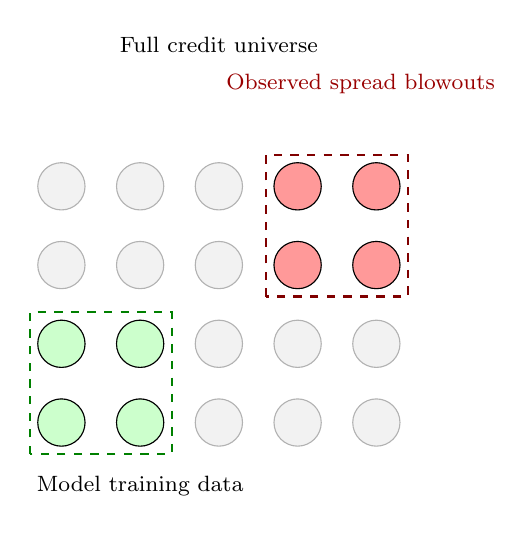
\begin{tikzpicture}[
      model/.style={circle, draw=black, fill=green!20, minimum size=0.6cm},
      blowout/.style={circle, draw=black, fill=red!40, minimum size=0.6cm},
      neutral/.style={circle, draw=black!30, fill=gray!10, minimum size=0.6cm},
      every node/.style={font=\scriptsize}
  ]
  
  % Credit universe grid (5x4)
  \foreach \x in {0,1,2,3,4} {
      \foreach \y in {0,1,2,3} {
          \node[neutral] (n\x\y) at (\x, \y) {};
      }
  }
  
  % Model training region (bottom-left 2x2)
  \foreach \x in {0,1} {
      \foreach \y in {0,1} {
          \node[model] at (\x, \y) {};
      }
  }
  
  % Blowout region (top-right 2x2)
  \foreach \x in {3,4} {
      \foreach \y in {2,3} {
          \node[blowout] at (\x, \y) {};
      }
  }
  
  % Labels
  \node[align=left, font=\footnotesize] at (1, -0.8) {Model training data};
  \node[align=left, font=\footnotesize, text=red!60!black] at (3.8, 4.3) {Observed spread blowouts};
  \node[align=left, font=\footnotesize] at (2, 4.8) {Full credit universe};
  
  \draw[dashed, thick, green!50!black] (-0.4, -0.4) rectangle (1.4, 1.4);
  \draw[dashed, thick, red!50!black] (2.6, 1.6) rectangle (4.4, 3.4);
  
  \end{tikzpicture}
  \caption{Spread Blowout Occurred Outside Model Coverage: The model was trained on credit names in calm regimes (green), but the shock hit an unmodeled set of issuers (red).}
\end{figure}

\medskip

The AI never flagged this because it had learned from historical data that IG bonds and oil weren’t highly correlated.  
It assumed the CDS short would \textit{offset} the oil exposure.

Instead, both positions bled simultaneously.

The selling fed on itself.  
As prices dropped, margin requirements recalibrated mid-day.  
Auroras’s model, trained on low-volatility environments, continued recommending small rebalances instead of issuing 
a halt.

\begin{itemize}
  \item By 2:30 p.m., Arcadia had received four sequential margin calls.  
  \item By 3:15 p.m., they had begun liquidating equity positions to cover margin on the credit book.  
  \item By 4:00 p.m., they were locked out of their own OMS, triaging via phone.
\end{itemize}

Aurora issued a severity alert, but only after 89\% of daily liquidity had already dried up.

\subsection{The Day Arcadia Unwound}

The next morning, Arcadia’s portfolio \textbf{NAV was down 47\%}.

\medskip

\begin{HistoricalSidebar}{The Cult of NAV}

  \textbf{NAV}, or \textit{Net Asset Value}, was originally a mundane accounting tool — a snapshot of what a 
  portfolio was worth if you sold everything, paid off the debts, and called it a day.

  \medskip
  
  But in the late 20th century, NAV became something more: a totem of institutional legitimacy. Hedge funds, 
  mutual funds, venture portfolios — all started tethering their credibility to this fluctuating number, 
  updated obsessively, audited reluctantly, and weaponized politically.

  \medskip
  
  When Arcadia’s NAV dropped 47\% overnight, it wasn’t just a financial event. It was a reputational implosion — 
  the kind that could empty boardrooms, evaporate term sheets, and trigger frantic calls from LPs who didn’t 
  remember what they signed up for.

  \medskip
  
  NAV pretends to be objective. But it’s part oracle, part theater: a number everyone believes in, until they 
  don’t — and then it becomes the reason they run.
  
\end{HistoricalSidebar}

\medskip

Nearly half the fund’s value was incinerated before breakfast.

There was no breaking news alert. No Bloomberg headline. Just an eerie stillness across desks and terminals.  
Slack channels turned quiet. Risk dashboards failed to load.  
Models that once converged now spat out nonsense (i.e. prices with no bids, implied volatilities that made no sense, etc...).  
Some assets had simply stopped trading. Others had no consensus price at all.  
One trader stared at an IG bond trading 12 points below model. Another muttered, “This looks like '08 pricing,” but no one 
corrected him.

\textbf{Two of their counterparties had already seized collateral.}

There were no discussions. Just automatic clauses kicking in.

One bank pulled pledged Treasuries and offloaded them into a fragile market.  
Another swept the cash reserve account without a word, citing “collateral optimization” language buried in Schedule A.  

Arcadia’s legal team tried to confirm if the counterparties had breached any protocols.  
Compliance quietly responded: “No... the protocols are working exactly as designed.”

Because these weren’t partnerships.  
These were \textit{derivative contracts}... and when the numbers move, the hands move with them.  
The CDS variation margin engine recalculated, and the collateral calls refreshed hourly.  

Behind the scenes, clearing brokers began tightening terms, demanding same-day margin and marking down previously AAA paper.  
Their prime desk pinged twice. Then went dark.

Arcadia still technically existed.  
But their positions were being unwound... not by strategy, but by clause.  
And every asset sold into that environment was fuel on the fire.

\textbf{By Friday, redemption requests hit \$1.2 billion.}

\medskip

\begin{figure}[H]
  \centering
  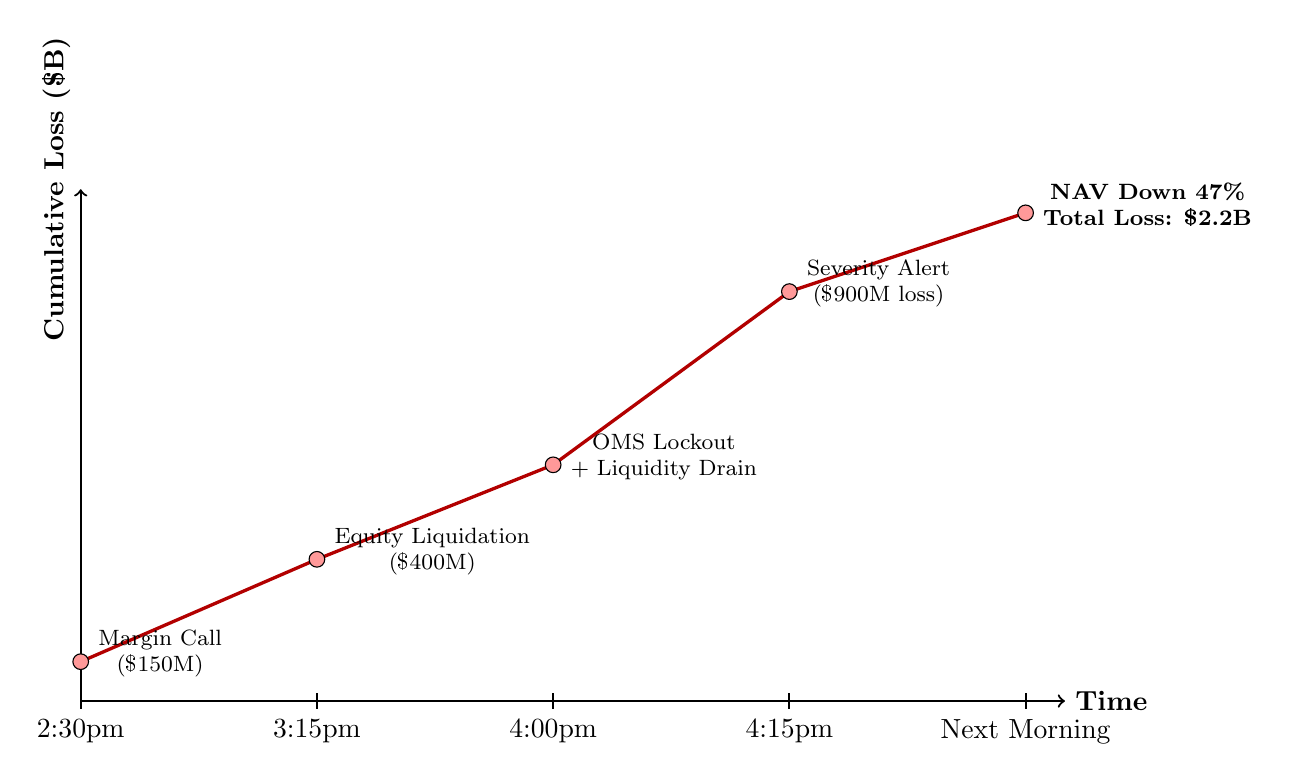
\begin{tikzpicture}[
    scale=1,
    axis/.style={thick, ->},
    event/.style={font=\footnotesize, align=center},
    loss/.style={circle, fill=red!40, draw=black, minimum size=4pt, inner sep=2pt}
  ]
  
  % Axes
  \draw[axis] (0,0) -- (12.5,0) node[right] {\textbf{Time}};
  \draw[axis] (0,0) -- (0,6.5) node[above, rotate=90] {\textbf{Cumulative Loss (\$B)}};
  
  % Time markers
  \foreach \x/\label in {
    0/2:30pm,
    3/3:15pm,
    6/4:00pm,
    9/4:15pm,
    12/Next Morning
  } {
    \draw[thick] (\x,0.1) -- (\x,-0.1) node[below] {\label};
  }
  
  % Loss line
  \draw[very thick, red!70!black]
    (0,0.5) 
    -- (3,1.8) 
    -- (6,3.0) 
    -- (9,5.2)
    -- (12,6.2);
  
  % Dots on line
  \node[loss] at (0,0.5) {};
  \node[loss] at (3,1.8) {};
  \node[loss] at (6,3.0) {};
  \node[loss] at (9,5.2) {};
  \node[loss] at (12,6.2) {};
  
  % Annotations
  \node[event, anchor=west] at (0.1,0.6) {Margin Call\\(\$150M)};
  \node[event, anchor=west] at (3.1,1.9) {Equity Liquidation\\(\$400M)};
  \node[event, anchor=west] at (6.1,3.1) {OMS Lockout\\+ Liquidity Drain};
  \node[event, anchor=west] at (9.1,5.3) {Severity Alert\\(\$900M loss)};
  \node[event, anchor=west] at (12.1,6.3) {\textbf{NAV Down 47\%}\\\textbf{Total Loss: \$2.2B}};
  
  \end{tikzpicture}
  \caption{Escalating Cumulative Loss: Arcadia's collapse unfolded in phases, each compounding the damage.}
\end{figure}

\medskip

By 10:12 a.m., their fund administrator still hadn’t updated the NAV file.  
Because no one knew what the portfolio was worth anymore.  
They only knew what was left to seize.

There was no warning. There was just automated triggers deep in the clearing system. The custodians didn’t call. 
The lawyers didn’t wait. The terms were predefined, and the math was cold. Arcadia's most liquid, high-quality 
assets were now gone — transferred without negotiation, in accordance with the agreements no one had re-read in years.

The machine learning system hadn’t caught the spiral because the model itself was \textbf{too simple}.

It had been trained on a world that was calm, segmented, and statistically clean. A world where \textit{oil 
prices and corporate bonds} danced to different rhythms. Where energy volatility was assumed to be independent 
from investment-grade credit.

It saw that — historically — these two variables didn’t move together. So it treated them like strangers at a 
party: in the same room, maybe, but not interacting.

But markets don’t behave like that under stress. \textbf{Under stress, independence collapses.} The wall 
between risk factors disappears. Everyone rushes for the same exits — at the same time.

\textbf{It’s like training a weather model on sunny days.}

You feed it years of calm skies and scattered clouds, and it learns that rain is rare and local. Then one 
day, a tropical storm forms offshore, but the model doesn’t recognize it. It doesn’t even have a word for 
``hurricane.''

So it keeps predicting a warm breeze... even when the roof blows off.

\medskip

\begin{figure}[H]
  \centering
  \resizebox{\textwidth}{!}{%
  \begin{tikzpicture}[
    node distance=1.2cm and 2.2cm,
    every node/.style={font=\small},
    box/.style={draw, rounded corners, minimum width=3.8cm, minimum height=1.2cm, align=center, fill=gray!10},
    arrow/.style={->, thick}
  ]
  
  % Top layer (assumptions)
  \node[box] (data) {Narrow Training Data\\(Low-volatility, stable regime)};
  \node[box, right=of data] (assumption) {Learned Historical\\Decorrelation};
  \node[box, right=of assumption] (blindspot) {No Calibration for\\Joint Stress Events};
  
  % Middle layer (stress response)
  \node[box, below=2cm of blindspot] (shock) {Oil Collapse \& CDS Spread Blowout\\Ignored as Uncorrelated};
  \node[box, left=of shock] (margin) {Margin Calls Trigger Forced Selling};
  \node[box, left=of margin] (amplify) {Selling Widens Spreads\\Triggers More Margin Calls};
  
  % Bottom layer (outcomes)
  \node[box, below=2cm of margin] (late) {AI Issues Alert\\After 89\% Liquidity Is Gone};
  \node[box, right=of late, fill=red!20] (result) {\textbf{Catastrophic Losses}\\Portfolio -47\%};
  
  % Arrows (top layer)
  \draw[arrow] (data) -- (assumption);
  \draw[arrow] (assumption) -- (blindspot);
  
  % Arrows (top → middle)
  \draw[arrow] (blindspot.south) -- (shock.north);
  \draw[arrow] (shock) -- (margin);
  \draw[arrow] (margin) -- (amplify);
  
  % Arrows (middle → bottom)
  \draw[arrow] (amplify.south) -- (late.north);
  \draw[arrow] (late) -- (result);
  
  \end{tikzpicture}
  }
  \caption{Three-stage breakdown: flawed assumptions, failure under stress, and financial collapse.}
\end{figure}
  
\medskip

The real failure wasn’t complexity.  It was a blind trust in patterns that only held when nothing went wrong.

Investors weren’t asking questions. They were getting out. Pension funds. University endowments. Family offices. 
The ones who had praised the fund's “adaptive AI risk engine” in the good years now submitted terse, and 
one-line notices.

The lines on the redemption ledger didn’t come from fear. They came from strategy. Nobody wanted to be the 
last LP left holding the bag when the final markdown came.

Inside Arcadia, the illusion of control collapsed faster than the portfolio.

One PM tried to open a spreadsheet but stared blankly at the loading icon. Another whispered, 
“Do we even know what we own right now?” A third walked out and didn’t come back.

The Irony? The AI dashboard was still green. \textit{But the lights in the office were turning off.}

\medskip

\begin{HistoricalSidebar}{Systems Thinking and the Feedback Loop Trap}

  %\textbf{Origin: The Rise of Systems Thinking.}  
  In the mid-20th century, fields as diverse as biology, engineering, and military planning converged 
  around a shared insight: complex systems behave in ways that cannot be understood by examining individual 
  parts in isolation. This gave rise to \textit{cybernetics} — the study of feedback, control, and 
  communication in systems — pioneered by Norbert Wiener and later extended by figures like Jay Forrester 
  at MIT.

  \medskip
  
  %\textbf{Positive vs. Negative Feedback.}  
  Systems thinking distinguished between two types of feedback:  

  \medskip

  \begin{itemize}
    \item \textbf{Negative feedback} dampens volatility -- e.g., a thermostat turning off heat once a set 
    temperature is reached.  
    \item \textbf{Positive feedback} amplifies shocks —- e.g., margin calls triggering sales, which trigger 
    more margin calls.
  \end{itemize}

  \medskip
  
  %\textbf{Finance Discovers Feedback — Too Late.}  
  Despite its relevance, systems thinking arrived late to finance. Classical economic models favored 
  linearity, equilibrium, and independence. It wasn’t until repeated crises (from portfolio insurance in 
  1987, to LTCM in 1998, to the 2008 liquidity spiral) that feedback loops were recognized as systemic threats.

  \medskip
  
  %\textbf{The Arcadia Collapse: A Textbook Feedback Spiral.}  
  The model failed not because it lacked data, but because it lacked \textit{structure}. It treated 
  historical correlations as if they were laws. It did not treate them as emergent properties of a fragile, 
  interconnected system. Therefore, when oil crashed, Arcadia’s hedges amplified rather than absorbed losses. 
  Liquidity dried up.  The feedback loop ignited.  

  \medskip
  
  \textbf{And the model?}  
  It kept recommending ``rebalance.''
  As if you could rearrange deck chairs on a burning ship.
  
  \medskip

  \begin{center}
  \textit{In systems with positive feedback, stability is not the norm... it’s a temporary illusion.}
  \end{center}
  
\end{HistoricalSidebar}

\medskip

\subsection{The Audit}

When the dust settled, the auditors arrived.
The auditors did not arrive with alarms or outrage. They arrived with clipboards, spreadsheets, and institutional detachment.
They didn’t need to ask who was responsible. The signatures were already timestamped. The logs were immutable. 
The collapse was self-documenting.

Then came the regulators.
They were slower, but hungrier.
They didn’t come to fix the system. They came to write the story... and to make sure someone’s name filled 
the footnotes of failure. They asked questions that sounded simple but weren’t.


``Who approved the leverage?'' asked the Senior Forensic Analyst from the SEC, eyes steady over rimless glasses.

David sat with his hands folded, palms damp. ``The decision to raise the exposure cap came from the portfolio team. I wasn’t involved in that approval.''

The analyst didn’t nod. He just blinked once. ``But you provided the risk assessment, correct?''

David hesitated. ``I prepared the system output. Yes.''

``Specifically the version dated three days before the exposure increase?''

``Yes.''

The analyst flipped through a binder, stopping at a page with highlighted sections. ``According to this, the model flagged an increase in cross-asset volatility. Why was that column excluded in the final risk memo sent to Investment Oversight?''

David felt the heat rise in his neck. ``We were still calibrating the signal. At that point, it had high sensitivity and was generating noise—false positives.''

``And who made the decision to suppress it?''

David paused. ``Technically, I did.''

``Why?''

He swallowed. ``Because I didn’t want it to distract from the broader findings. The rest of the model showed acceptable thresholds.''

The analyst looked up. ``Acceptable under what assumptions?''

``Under calm regime behavior. Which, at the time—''

``—was already breaking down in commodity markets,'' the analyst interrupted gently. ``You removed the only indicator showing early instability. Why?''

David shifted in his seat. ``We thought it was a blip. Noise.''

``Did you note that in the report?''

``No. It didn’t seem material at the time.''

``Yet it was material enough to suppress?''

The room fell quiet.

The analyst tapped his pen once on the table. ``So, when Investment Oversight pushed the leverage increase, they were acting under the impression that all volatility indicators were neutral.''

David didn’t answer.

``And the one flag that wasn’t neutral — the one warning sign — was missing because you thought it might cause confusion.''

David looked down. ``I didn’t mean to mislead anyone.''

``Intent isn't the question,'' the analyst said. ``The question is whether your report enabled a decision that should never have been made.''

Another pause. Then:

``Mr. Morales,'' he continued, ``your name appears on the approval workflow. Not as decision-maker, but as validator. Your initials are here—right under the model output. Do you dispute that?''

David stared at the page.

``No,'' he said quietly. ``I don’t dispute that.''

``Thank you,'' the analyst said, and closed the binder with a soft click.

``That will do for now.''

\medskip

\begin{HistoricalSidebar}{The SEC and the Theater of Responsibility}

  Founded in the wake of the 1929 crash, the U.S. Securities and Exchange Commission (SEC) was designed as both 
  watchdog and confessor. It was designed to be part enforcement arm, and part national conscience for financial markets.

  \medskip
  
  Its mandate is simple: protect investors, ensure fair markets, and hold those accountable who threaten either. 
  But the execution is rarely so clean.

  \medskip
  
  In scenarios like David’s, the SEC doesn't storm the gates with sirens. It arrives in tailored suits and 
  calibrated language, interested less in guilt than in \textit{who signed what, when}. It reconstructs the internal 
  machinery: approval chains, suppressed signals, reporting thresholds — all to trace how a decision came to look inevitable.

  \medskip
  
  By the time the SEC enters the room, the damage is already done. Its job is to illuminate the moment it became 
  irreversible, to identify who, and hold the flashlight on them.
  
\end{HistoricalSidebar}

\medskip

``Why wasn’t the risk flagged?'' asked the Deputy Director of Risk Oversight from the Office of Systemic Risk.

His voice was calm, but he was already circling the failure — not of markets, but of \textit{detection}.

David took a beat. ``It depends which risk you’re referring to.''

``The synthetic credit tranche that ruptured three liquidity pools in under ninety minutes.''

David exhaled slowly. ``That product was flagged — in internal simulations. We just didn’t escalate it.''

``Why not?''

``The model showed instability only in certain stress-paths. And only when run at the 95th percentile sensitivity. Leadership considered that noise.''

``Did you?''

David hesitated. ``I thought it needed more time. The signal hadn’t stabilized.''

``And in the meantime, the exposure increased by 31\%.''

``I wasn’t in charge of allocations.''

``No,'' the Deputy Director said. ``But your report was cited as justification in the allocation memo.''

David blinked. ``I wasn’t aware of that.''

``Page 4, footnote 2. They reference your summary of model results and cite the volatility corridor as ‘within tolerance.’ Was it?''

David looked down. ``Only if you exclude derivative spillover effects. Which I hadn’t tested yet.''

``So you signed off on a model summary that didn’t include derivatives — even though the product in question was synthetic credit?''

``We were on a compressed timeline. There was pressure to deliver a greenlight framework by end-of-quarter.''

``From whom?''

``Multiple stakeholders.''

``Can you name them?''

``I'd prefer not to speculate.''

``You don’t need to speculate, Mr. Morales. You need to remember.''

A silence stretched — not hostile, but surgical.

``Let me put it another way,'' the Deputy Director said, folding his hands. ``You were responsible for identifying unstable pathways in Aurora’s credit engine. And yet, the most dangerous path — the one that actually unfolded — wasn’t flagged, wasn’t communicated, and wasn’t contained.''

``The model wasn’t broken,'' David said quietly. ``It just wasn’t finished.''

The Director nodded slowly. ``Neither was the crisis.''

``Thank you,'' he said, closing his folder. ``That will be all for now.''

\medskip

\begin{HistoricalSidebar}{The Office of Systemic Risk --- After the Crash, the Cartographer}

  The \textbf{Office of Systemic Risk}, operating under the Financial Stability Oversight Council (FSOC), 
  was created by the Dodd–Frank Act in 2010. It is not a market regulator, but a mapmaker of collapse.

  \medskip
  
  Its mandate wasn’t to monitor firms individually, but to identify threats that emerge when interlocking 
  systems --- funds, models, margin calls, and political pressures --- align catastrophically. In other words: 
  not \textit{who} failed, but \textit{how} the system was already wired to fail.

  \medskip
  
  In cases like Aurora, the Office doesn’t arrive looking for fraud. It arrives looking for fragility that 
  was normalized — risks that were technically visible, but socially invisible. Often, the most damaging 
  decisions were made with clean hands and plausible models.

  \medskip
  
  The Office’s investigators specialize in tracing these moments: where a suppressed flag or a downgraded 
  simulation quietly mutated into systemic exposure. Their job isn’t to prevent the last crash. It’s to 
  draw the blueprint for the next one, and to ask why no one sounded the alarm when the walls were 
  already shaking.
  
\end{HistoricalSidebar}

\medskip


``Where’s the board memo?'' asked the man in the dark suit — Special Counsel for the Congressional Subcommittee 
on Financial Accountability. He spoke plainly, but each word felt like it had been cleared with legal counsel.

David looked down at the folder in front of him. ``Which memo, exactly?''

``The one documenting leadership’s awareness of the leverage adjustment and cross-product exposure. The one that 
should’ve gone to the Risk and Audit Committee in Q2. We’ve reviewed the board packets. It’s not there.''

David cleared his throat. ``If it wasn’t escalated, that would’ve been Compliance’s responsibility.''

The counsel nodded once. ``So you didn’t draft a briefing note?''

``No formal memo, no. We discussed elements of it in working groups.''

``Any minutes from those meetings?''

``Possibly. Not all sessions were minuted.''

``Were any slides presented to executive leadership?''

``There were slides,'' David said. ``But they were high-level.''

``How high-level?''

``Portfolio allocation bands. General trends. Scenario ranges.''

``Any mention of the synthetic tranche correlation drift?''

David hesitated. ``Not explicitly, no.''

The counsel glanced down at a binder. ``Your team internally referred to that drift as `uncontained contagion 
velocity’ in a Slack thread dated April 17th. Would you say that rises to the level of board visibility?''

David blinked. ``That was informal language.''

``So the board received a sanitized version?''

``They received a \textit{strategic} summary,'' David said carefully.

``Without the risks.''

``Without the emerging anomalies,'' he corrected.

``And who decided those anomalies didn’t merit inclusion?''

``That would have been a judgment call across multiple leads.''

``But your name is listed as the document owner on the draft outline. Yes?''

David didn’t answer.

The counsel didn’t press — not directly.

``Mr. Morales, when boards are kept in the dark, we investigate whether it was by accident or by design. Right now, 
it looks like your team filtered the light. That’s not a modeling issue. That’s governance.''

He closed the folder.

``And the next question will be: who gave permission... and who gave cover.''

\medskip

\begin{HistoricalSidebar}{The Congressional Subcommittee on Financial Accountability}

  The \textbf{Congressional Subcommittee on Financial Accountability} is less a financial authority and more a political 
  lens — trained on moments when markets fail and someone, somewhere, must be made to answer.

  \medskip
  
  Historically activated after high-visibility collapses --- Enron (2001), Lehman Brothers (2008), Archegos (2021) --- the 
  Subcommittee is tasked with tracing breakdowns in oversight, disclosure, and board governance. Its focus isn’t technical 
  modeling or trading algorithms; it’s \textit{who knew what, when}, and why warnings were buried, softened, or ignored.

  \medskip
  
  Unlike regulatory bodies such as the SEC or FSOC, which prioritize structural risk, the Subcommittee pursues political 
  and ethical accountability. It doesn’t ask if the system failed. It asks whether people in positions of fiduciary trust 
  failed to act.

  \medskip
  
  In hearings, terms like ``strategic ambiguity,'' ``sanitized summaries,'' and ``decision path opacity'' become signals 
  of willful negligence. In this theater, plausible deniability often reads as intent.

  \medskip
  
  The result may not be criminal indictment. Howeverr, reputational collapse begins here.
  
\end{HistoricalSidebar}

\medskip

\subsection{The Investigation}

And then the subpoenas.
Each one a bullet with a return address.
Not everyone got one. Just enough to split the room.
Colleagues stopped making eye contact. PR firms started drafting pre-denial denials. DMs were deleted. Laptops were “misplaced.” Someone called a lawyer. Someone else called their parents.

Everyone still inside the building understood the game now:
The collapse was over.
The reckoning had begun.

The investigation was clinical, and methodical.
There were no accusations. No raised voices.
Just quiet meetings behind closed doors,
and inboxes filling with calendar invites marked “Confidential.”

They didn’t start with blame.
They started with logs.
Time-stamped outputs. Deployment metadata. Git histories.
Everything left a trail — and the trail, like all trails, led somewhere.

They traced the failure back to the model.
The model that hadn’t flagged the risk.
The model that weighted the wrong variables, at the wrong time, in the wrong market regime.

They traced the model back to the deployment.
The rushed rollout two weeks ahead of schedule.
The feature freeze that had been quietly ignored.
The patch that was never peer-reviewed because “we needed velocity.”

They traced the deployment back to the sign-off.
The approval checkpoint. The final green light.
The digital rubber stamp that turned code into consequence.

And the sign-off?

\textbf{David’s initials.}

Three letters in the lower right corner of the commit approval screen.
A routine click, made after a long day, probably during a Zoom call.
No malicious intent. No recklessness.
Just the ordinary negligence of someone who believed the system was stable —
because it always had been.

Until it wasn’t.

\medskip

\begin{HistoricalSidebar}{Knight Capital: The \$440 Million Glitch}

  On August 1, 2012, Knight Capital Group, a major player in U.S. equities trading,  
  experienced a catastrophic software malfunction. A faulty deployment activated obsolete code,  
  triggering a dormant feature flag and causing the firm’s automated systems to execute errant trades at lightning speed.  
  Within 45 minutes, Knight had amassed unintended positions totaling approximately \$7 billion, resulting in a  
  loss of \$440 million.
  
  \medskip
  
  After an investigation, regulators found no willful misconduct. The engineers had followed protocol.  
  Sign-offs had been documented. Deployment processes had been technically satisfied.  
  There was no scapegoat. No intentional wrongdoing.  
  The disaster had emerged from a tragic convergence of overlooked legacy code and system complexity—  
  an error that might have happened to anyone.
  
  \medskip
  
  But it could have gone differently.
  
  \medskip
  
  Had the engineers skipped a sign-off, failed to document a test, or deviated from internal controls,  
  the finding could have shifted from “no fault” to negligence—or worse, willful misconduct.  
  And in securities law, there’s a thin, terrifying line:  
  Most corporate indemnification protects you from mistakes.  
  But it stops short at two critical points:  
  \textbf{willful misconduct} and \textbf{gross negligence}.
  
  \medskip
  
  In highly regulated industries, you don’t need to commit fraud to face prosecution.  
  You only need to fail to do enough.
  
  \medskip
  
  In the wake of the collapse, new regulations were enacted. Additional verification steps mandated.  
  Audit trails hardened. Controls tightened.  
  But the deeper lesson remained unsettling:  
 
  \begin{quote}
  Sometimes, even with due diligence, the system can still break.  
  And if you’re standing too close to the fault line when it does,  
  there’s no guarantee the legal shield will hold.
  \end{quote}
  
\end{HistoricalSidebar}
  
\medskip

The district attorney didn’t find coercion.  
There were no emails instructing them to skip validation.  
There were no memos ordering corners cut.  

Hart had never told them to ship an unvalidated model.  
Hart had simply praised their speed.  
Hart had simply reassured their doubts.  
Hart had made the window of opportunity feel fleeting.  
Hart had framed the risk as reputational, not systemic.

David hadn’t been ordered.  
David had complied.  
David had complied voluntarily. David had complied eagerly.  
David complied without ever realizing he was making a choice at all.

By the time the indictments were drafted, every thread of formal responsibility led back to Aurora.  
The signatures.  
The approvals.  
The compliance checklists, half-complete and timestamped in their own systems.

Hart hadn’t touched the model.  
Hart hadn’t approved the launch.  
Hart hadn’t held an official role at Aurora at all.

He didn’t need to.

The funnel had worked.

The web was theirs.  
But the liability was Aurora’s.

And Hart?  
Hart was already pouring another drink.  
Hart was already sketching another napkin.  
Hart was already leaning in close to the next founder, and  
smiling warmly as if nothing had ever happened.

\subsection{The Aftermath}

In the weeks before sentencing, David’s world narrowed to court dates, lawyer meetings, and restless 
nights in an apartment that no longer felt like home.

Emma was supportive. At least, that’s how it appeared.  
She brought him meals. Sat quietly beside him. Held his hand when the lawyers left grim updates on the voicemail.

One evening, she placed a hand gently on his shoulder.  
“I’ll wait for you,” she promised softly.  

Her smile was warm. Her smile was reassuring. Her smile was almost maternal.  

“It won’t be hard,” she added, with a calm and unbothered voice.
“Serena and Hart have been so kind. They’re making sure I’m not alone through all this.”

She kissed his forehead.

And in that moment, David realized that 
Emma wasn’t waiting for him.  
Emma was already somewhere else.  
Emma was somewhere he didn't belong.

By the time the sentence was handed down,  
David understood something he hadn’t in the beginning. 

What happens in the boardroom doesn't stay in the boardroom.  It follows you home.
